\documentclass[a4paper,8pt,twocolumn]{extarticle}
\usepackage[utf8]{inputenc}
\usepackage{graphicx}
\usepackage[center, font=small]{caption}
\usepackage[english]{babel}
\usepackage[top=2.5cm, bottom=2.5cm, left=2.5cm, right=2.5cm]{geometry}

%---------------------------------------------
% Font packages
%---------------------------------------------
\usepackage{lmodern}
% \usepackage{concmath}
% \usepackage{cmbright}
% \usepackage{kpfonts}
% \usepackage[adobe-utopia]{mathdesign}
% \usepackage{fouriernc}
\usepackage[T1]{fontenc}

%---------------------------------------------
% Math environment packages & command
%---------------------------------------------
\usepackage{amsmath}
\usepackage{amssymb}
\usepackage{array}
% \usepackage{mathrsfs}
\usepackage{array}
% \def\sgn{\mathop{\rm sgn}\nolimits} 
% \usepackage{bbm}
\usepackage{schemabloc}

%---------------------------------------------
% item option
%---------------------------------------------
\renewcommand{\labelitemi}{-}

%---------------------------------------------
%HEADER & FOOTER
%---------------------------------------------
\usepackage{fancyhdr}
\pagestyle{fancy}

\renewcommand{\headrulewidth}{.15pt}
\fancyhead[C]{{\textsc{Multivariable Systems}}} 
\fancyhead[L]{Page \thepage \ of \pageref{LastPage}}
\fancyhead[R]{EL2520}

\renewcommand{\footrulewidth}{.15pt}
\fancyfoot[C]{\thepage} 
% \fancyfoot[L]{truc}
\fancyfoot[R]{EE -- Automatic Control}

\usepackage{lastpage}

%---------------------------------------------
% two column option
%---------------------------------------------
\setlength{\columnsep}{0.5cm}

%---------------------------------------------
% Table of content
%---------------------------------------------
\usepackage[colorlinks,linkcolor=black, citecolor=black]{hyperref}

%---------------------------------------------
% Opening
%---------------------------------------------
\title{Computer Exercice:\\ \textsc{Multivariable Systems}}
\author{Jean-Alix \textsc{David}, Kilian \textsc{Demeulemeester} \\ \texttt{\{jadavid,kiliande\}@kth.se}}

%---------------------------------------------
% Numerotation Handling
%---------------------------------------------
\setcounter{section}{2}
\usepackage[explicit]{titlesec}
% \titleformat{<command>}[<shape>]{<format>}{<label>}{<sep>}{<before>}[<after>]
\titleformat{\subsubsection}[hang]{\Large\normalsize\bfseries\centering}%
    {}{4pt}%
    {\dotfill\hspace{0.5cm}\emph{#1 \arabic{section}.\arabic{subsection}.\arabic{subsubsection}}\hspace{0.5cm}\dotfill} 

    \titleformat{\paragraph}[hang]{\footnotesize\bfseries\centering}{}{4pt}{\emph{#1}}
    %\titleformat{\paragraph}[hang]{\footnotesize\bfseries}{}{4pt}{\dotfill\hspace{0.5cm}\emph{#1}\hspace{0.5cm}\dotfill}
%---------------------------------------------
% Dummy text
%---------------------------------------------
\usepackage{lipsum}

%---------------------------------------------
% Item package option 
%---------------------------------------------
%\usepackage[shortlabels]{enumitem}
\newenvironment{shortitemize}{
    \begin{itemize}
        \setlength{\itemsep}{0pt}
        \setlength{\parskip}{0pt}
        \setlength{\parsep}{0pt}
    }{\end{itemize}}

\begin{document}

% Indent length
\setlength\parindent{0em}

\maketitle

%\tableofcontents

\begin{bfseries}
\emph{Abstract} -- 
Bla bla...
\end{bfseries}


\section{Exercises}

\subsection{Poles, zeros and RGA}

The system is modelized as a MIMO system with two inputs ($u_1 \& u_2$) and two ouputs ($y_1 \& y_2$).
The multivariable model with $2$ inputs and $2$ outputs is given by $Y(s) = G(s)U(s)$.
Depending on the settings of the valves -- minimum/maximum phase model -- we obtain different $G(s)$.
Each exercise in the following take care of the two settings.

\subsubsection{Exercise}
\paragraph{Minimum phase model}

The transfer matrix $G_{mp}(s)$ is:

$$G_{mp}(s) = \left(\begin{array}{cc} 
    \frac{.035}{s + .056} & \frac{.00046}{s^2 + .082 s + .0015} \\
    \\
    \frac{ .00044}{  s^2 + .073 s + .0011} & \frac{.030}{s + .052} \\
\end{array}\right)$$


Poles and zeros of the elements are given in the following table:

$$
\text{Poles}(G_{mp,i,j}(s)) = \left(\begin{array}{cc} -.056 & \left(\begin{array}{c} -.056\\ -.026 \end{array}\right) \\ \left(\begin{array}{c} -.052\\ -.021 \end{array}\right) & -.052 \\ \end{array}\right)
$$

$$\text{Zeros}(G_{mp,i,j}(s)) = \emptyset $$

\paragraph{Non-minimum phase model}

The transfer matrix $G_{nmp}(s)$ is:

$$G_{nmp}(s) = \left(\begin{array}{cc} 
    \frac{.021}{s + .051} & \frac{.0026}{s^2 + .14 s + .0044} \\
    \\
    \frac{ .0032}{ s^2 + .14 s + .0043} & \frac{.018}{s + .047} \\
\end{array}\right)$$

Poles and zeros of the elements are given in the following table:


$$\text{Poles}(G_{nmp,i,j}(s)) = 
\left(\begin{array}{cc} -.051 & \left(\begin{array}{c} -.086\\ -.051 \end{array}\right) \\ \left(\begin{array}{c} -.091\\ -.047 \end{array}\right) & -.047 \\ \end{array}\right)
$$

$$\text{Zeros}(G_{nmp,i,j}(s)) = \emptyset $$

\subsubsection{Exercise}

\paragraph{Minimum phase model}

Poles and zeros of the multivariable system in the minimum phase model case are:

$$
\text{Poles}(G_{mp}(s)) = 
    \left(\begin{array}{c}  
    -.056 \text{ (double)} \\
    -.052 \text{ (double)} \\
    -.021 \\
    -.026 \\
    \end{array}\right)
$$
$$
\text{Zeros}(G_{mp}(s)) = 
    \left(\begin{array}{c}
    -.0093 \\
    -.038 \\
    -.056 \\
    -.052 \\
    \end{array}\right)
$$

\paragraph{Non-minimum phase model}

Poles and zeros of the multivariable system in the non-minimum phase model case are:

$$
\text{Poles}(G_{nmp}(s)) = \left(\begin{array}{c} -.051 \text{ (double)}\\ -.047 \text{ (double)} \\-.091 \\ -.086\\ \end{array}\right)
$$
$$
\text{Zeros}(G_{nmp}(s)) = \left(\begin{array}{c} -.24\\ .059\\ -.051\\ -.047 \end{array}\right)
$$

We see that there is one zero of $G_{nmp}(s)$ is in the right-hand side of the complex plane.
Therefore the system is \emph{(indeed)} a non-minimum phase systems.
This system offers a gain in the wrong direction for rapid inputs: the cross over frequency should be small.

Using the rule of thumb defined in the course the bandwith limitation is :
$$
\omega_{BS} \leq \frac{z}{2} = .029
$$

% \subsubsection{Exercice}
The largest and smallest singular values for the system at different frequencies for the minimum phase model are visible on figure \ref{singvalue}.

\begin{figure}[h!b]
    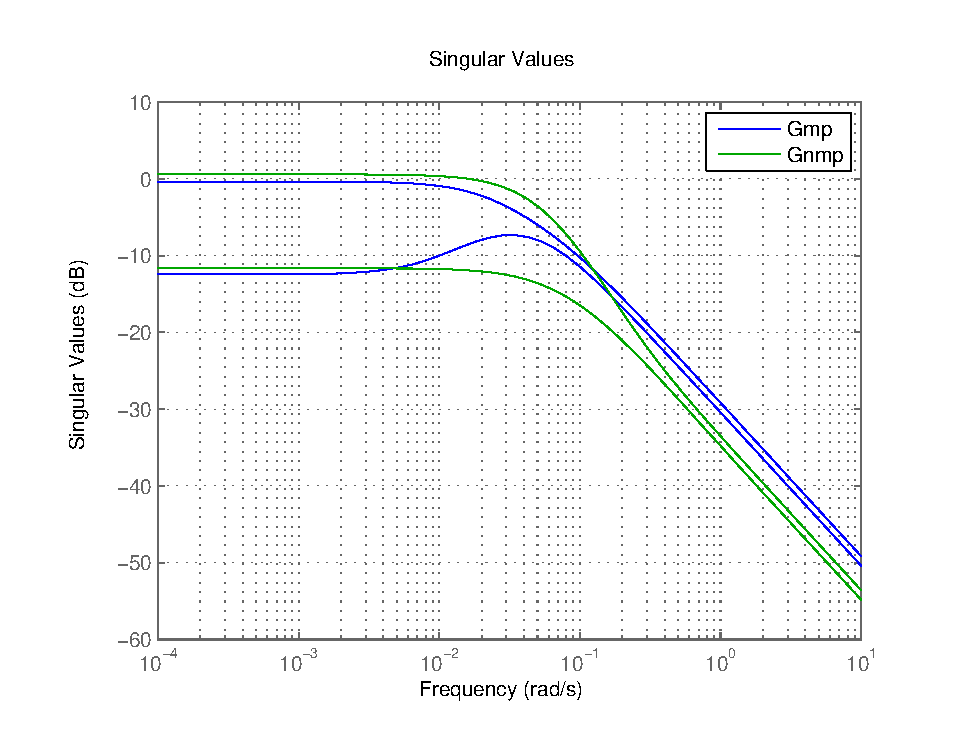
\includegraphics[width=\columnwidth]{fig/singvalue}
    \caption{$\underline{\sigma}(G(i\omega))$ and $\bar{\sigma}(G(i\omega))$ for the minimum phase model (blue) and the non-minimum phase model (green)}
    \label{singvalue}
\end{figure}

We have the following value for the $H_{\infty}$ norm of the systems:

$$\begin{array}{ccc}
    ||G||_{\infty,mp} =  .96
    & \text{ \textbf{and} } &
    ||G||_{\infty,nmp} = 1.1 
\end{array}
$$


% \subsubsection{Exercise}
\paragraph{Minimum phase model}

The RGA of the minimum phase system at frequency $0$ is:

\begin{multline*} 
    \text{RGA}(G_{mp}(0)) = \\
    G_{mp}(0) .* [G_{mp}^{-1}(0)]^T = \\
    \left(\begin{array}{cc} 1.6 & -0.56\\ -0.56 & 1.6 \end{array}\right)
\end{multline*}

Using the second rule of thumb expressed in the subject gives the following result:

\begin{center}
\begin{tabular}{|c|cc|}
    \hline
    & $u_1$ & $u_2$ \\ 
    \hline
    $y_1$ & $1$ & $0$ \\
    $y_2$ & $0$ & $1$ \\
    \hline
\end{tabular} \ \\ \ \\
($0$ -- avoid pairing, $1$ -- pairing possible).
\end{center}

\paragraph{Non-minimum phase model}

The RGA of the non-minimum phase system at frequency $0$ is:

\begin{multline*}
    \text{RGA}(G_{nmp}(0)) = \\ 
    G_{nmp}(0) .* [G_{nmp}^{-1}(0)]^T =  \\
    \left(\begin{array}{cc} -0.56 & 1.6\\ 1.6 & -0.56 \end{array}\right)
\end{multline*}

Using the second rule of thumb expressed in the subject gives the following result:

\begin{center}
\begin{tabular}{|c|cc|}
    \hline
    & $u_1$ & $u_2$ \\ 
    \hline
    $y_1$ & $0$ & $1$ \\
    $y_2$ & $1$ & $0$ \\
    \hline
\end{tabular} \ \\ \ \\
($0$ -- avoid pairing, $1$ -- pairing possible).
\end{center}


\textbf{Remark:} The two RGA matrix at frequency $0$ are symetrical. This seems legit since the alimentation of tanks 1 \& 4 is made by pump 1 and the alimentation of tanks 2 \& 3 is made by pump 2.

% \subsubsection{Exercise}

Figure \ref{step315} shows the step response of the systems (minimum phase \& non-minimum phase). 
As we can see the system is indeed coupled, with the same correlation as the one depicted by the properties of RGA.

% \subsubsection{Exercice}

The impact of each input can be measured as: $$\frac{|y_{\text{paired to } u_i}|}{|y_{\text{not-paired}}|}$$

We have the following relation:
\begin{shortitemize}
    \item Input (1):
$$\frac{|y_{1,m}|_\infty}{|y_{2,m}|_\infty} = \frac{.6}{.4} = 1.5 \leq \frac{|y_{2,nm}|_\infty}{|y_{1,nm}|_\infty} = \frac{.7}{.4} = 1.75$$  
    \item Input (2):
$$\frac{|y_{2,m}|_\infty}{|y_{1,m}|_\infty} = \frac{.6}{.3} = 2 \geq \frac{|y_{1,nm}|_\infty}{|y_{2,nm}|_\infty} = \frac{.6}{.4} = 1.5$$ 
\end{shortitemize}

This result can be sum up as:

\begin{center}
\begin{tabular}{|c|cc|}
    \hline
    Desired control & $y_1$ & $y_2$ \\ 
    \hline
    \multirow{2}*{$G_m(s)$} & Act on $u_1$ & Act on $u_2$ \\ 
                & \emph{Stronger} & \emph{Weaker}\\
                & \emph{coupling} & \emph{coupling} \\ 
    \hline
    \multirow{2}*{$G_{nm}(s)$} & Act on $u_2$ & Act on $u_1$ \\
             & \emph{Weaker} & \emph{Stronger}\\
             & \emph{coupling} & \emph{coupling} \\
    \hline
\end{tabular}
\end{center}

\begin{figure}[h!t]
    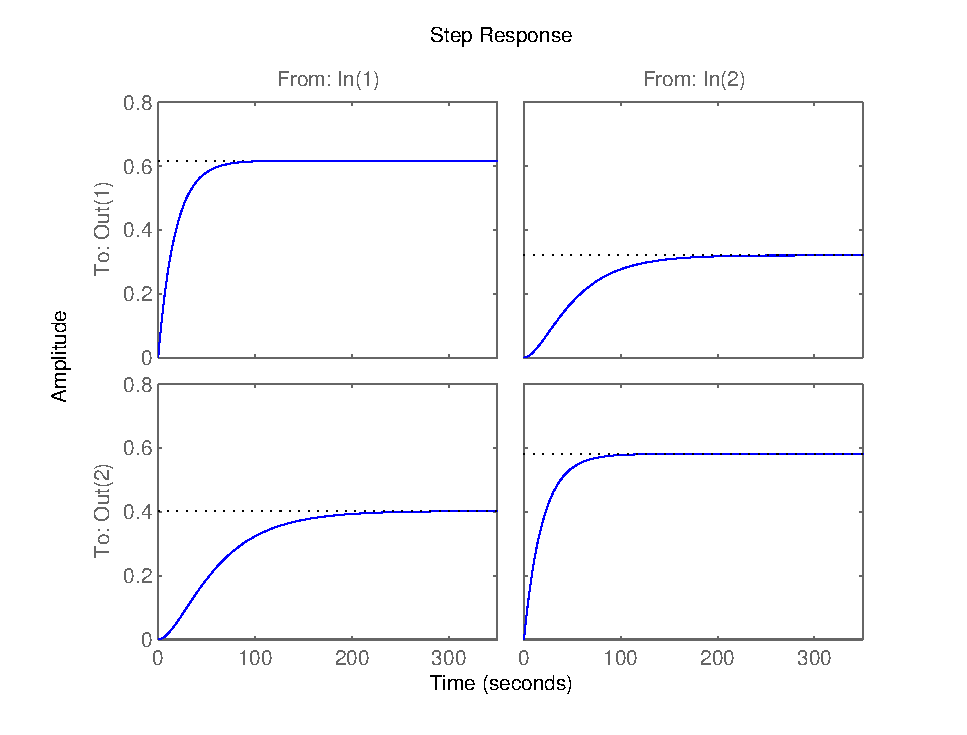
\includegraphics[width=\columnwidth]{fig/step315m}
    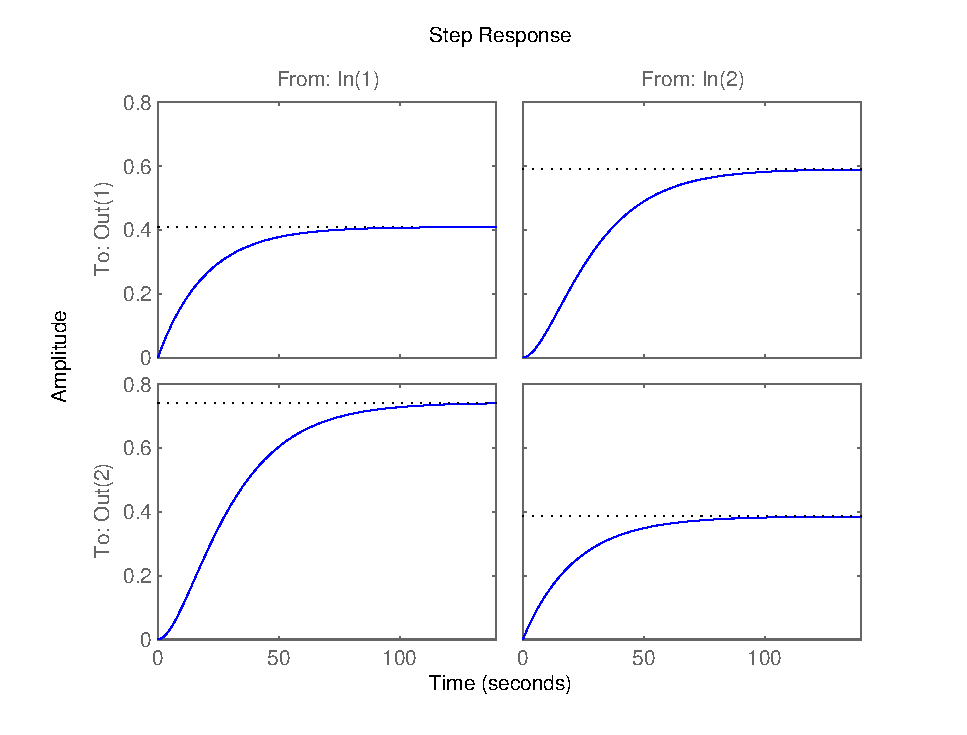
\includegraphics[width=\columnwidth]{fig/step315nm}
    \caption{Step responses of the systems}
    \label{step315}
\end{figure}



%\newpage

\subsection{Decentralized control}

% \subsubsection{Exercice}

The specification of the controlled system are the following:

\begin{shortitemize}
    \item Phase margin: $\varphi_m = \pi/3$
    \item Crossover frequency: 
        \begin{shortitemize}
            \item Minimum phase system: $\omega_{c,m} = .1$rad/s
            \item Non-minimum phase system: $\omega_{c,nm} = .02$rad/s
        \end{shortitemize}
\end{shortitemize}

As we can see $\omega_{c,nm} \leq .029$ (see Exercise 3.1.2). Therefore the RHP zero will not be a problem.

The controller are designed using the method depicted in the subject. 
We have the following values:

\begin{center}
    \begin{tabular}{|c|cc|}
        \hline
        & $f_1(s)$ & $f_2(s)$ \\
        \hline
        $F_{m}(s)$ & & \\
        $F_{nm}(s)$ & & \\
       \hline 
    \end{tabular}
\end{center}


% \subsubsection{Exercise}
\paragraph{Minimum phase model}

Figure \ref{singm} shows the maximum and minimum singular value of $S$ and $T$ as a function of the frequency. 
In this minimum-phase case, no restricting criteria was formulated regarding to $S$ and $T$.

\begin{figure}[h!t]
    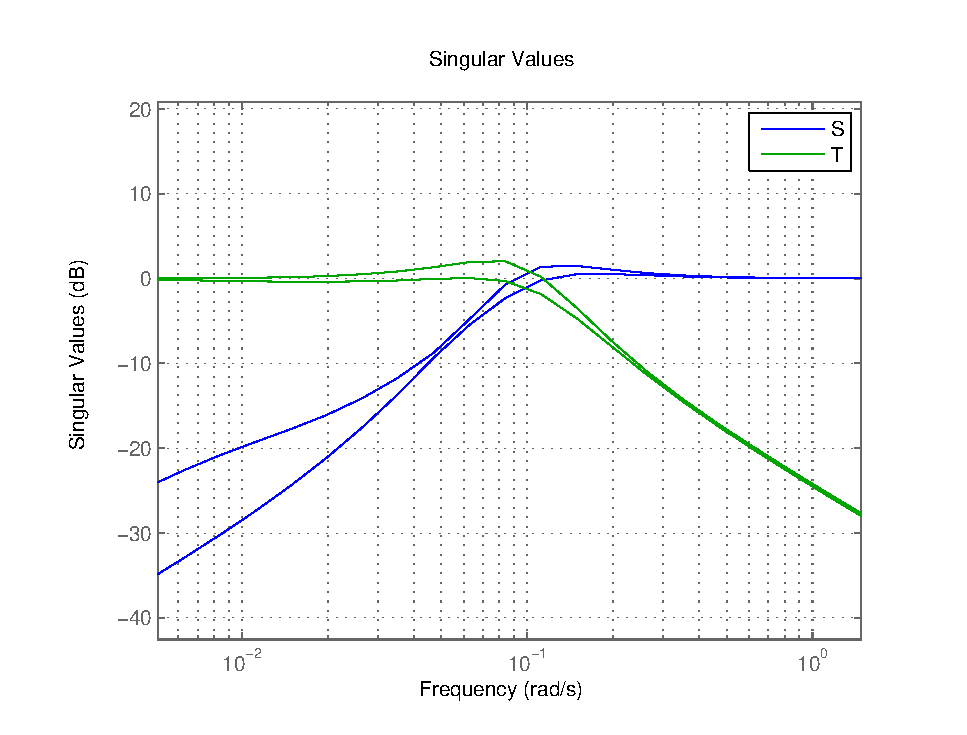
\includegraphics[width=\columnwidth]{fig/ST322m.eps}
    \caption{Singular values of $S$ and $T$ for the minimum phase system}
    \label{singm}
\end{figure}

\paragraph{Non-minimum phase model}


Figure \ref{singnm} shows the maximum and minimum singular value of $S$ and $T$ as a function of the frequency. 
In this non-minimum-phase case, since there is a RHP zero in the transfer matrix we had the following criteria regarding the bandwith limitation : $\omega_{BS} \leq 0.029$. This criteria is fulfilled.


\begin{figure}[h!t]
    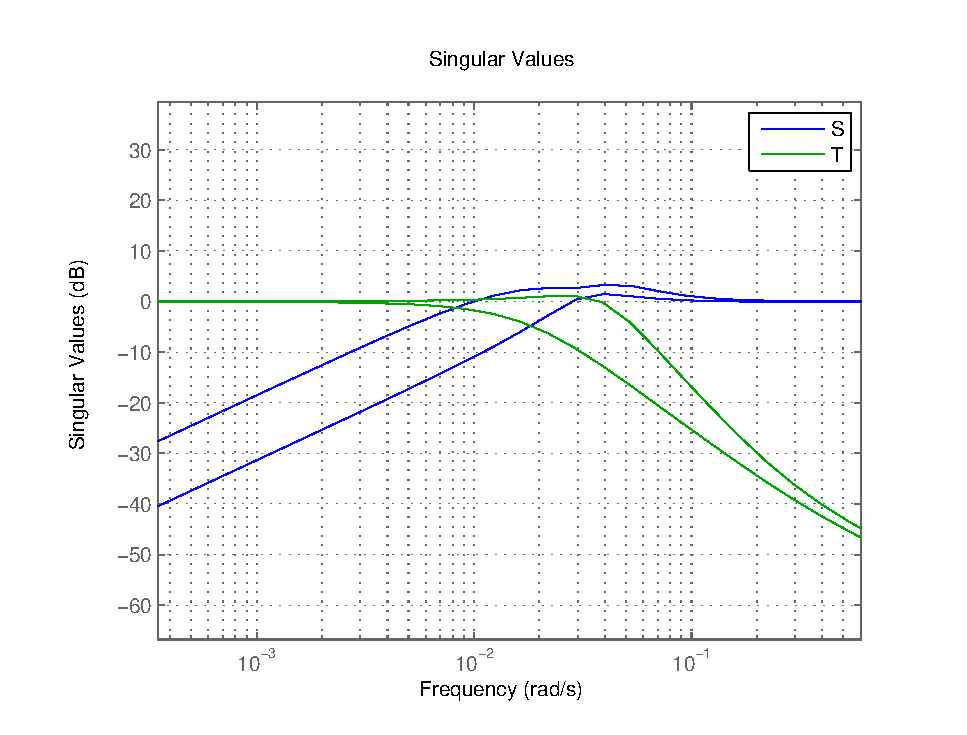
\includegraphics[width=\columnwidth]{fig/ST322nm.eps}
    \caption{Singular values of $S$ and $T$ for the non-minimum phase system}
    \label{singnm}
\end{figure}


% \subsubsection{Exercise}

Using simulink we simulate the closed-loop system for an input:
$$ r(t) = \left\{\begin{array}{rcl} r_1(t) & = & u_{t\geq 100} \\ r_2(t) & = & u_{t\geq 500} \end{array}\right.$$

\paragraph{Minimum phase model}

Figure \ref{simum} shows the output $y_1$ and $y_2$ of the closed-loop system in the minimum phase case. 
The control quality is the following: 
\begin{center}
\begin{tabular}{|c|ccc|}
    \hline
    & Overshoot& Overshoot& Rise\\ 
    & coupled & non-coupled & time \\
    \hline
    $y_1$ & $12\%$ & $0.1$ & $30$s  \\
    $y_2$ & $13\%$ & $0.1$ & $30$s  \\
    \hline
\end{tabular}
\end{center}

\begin{figure}[h!t]
    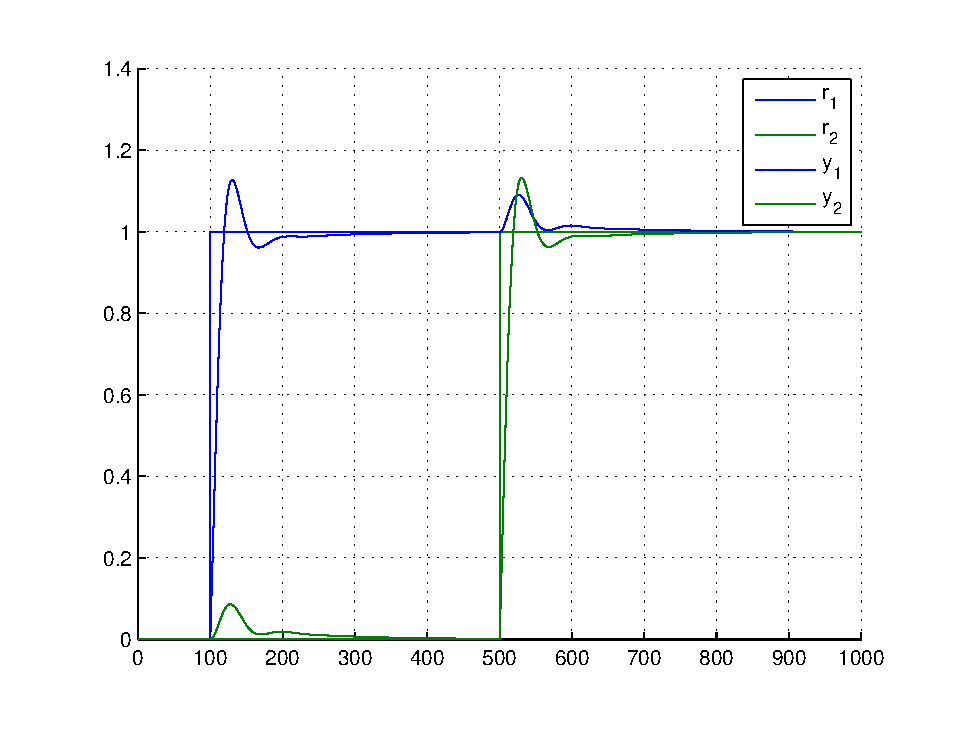
\includegraphics[width=\columnwidth]{fig/controlledouputm.eps}
    \caption{Response of the minimum phase system to $r(t)$}
    \label{simum}
\end{figure}

\paragraph{Non-minimum phase model}

Figure \ref{simunm} shows the output $y_1$ and $y_2$ of the closed-loop system in the non-minimum phase case. 
The control quality is the following: 
\begin{center}
\begin{tabular}{|c|ccc|}
    \hline
    & Overshoot& Overshoot& Rise\\ 
    & coupled & non-coupled & time \\
    \hline
    $y_1$ & $0\%$ & $0.5$ & $350$s  \\
    $y_2$ & $0\%$ & $0.35$ & $200$s  \\
    \hline
\end{tabular}
\end{center}

\begin{figure}[h!t]
    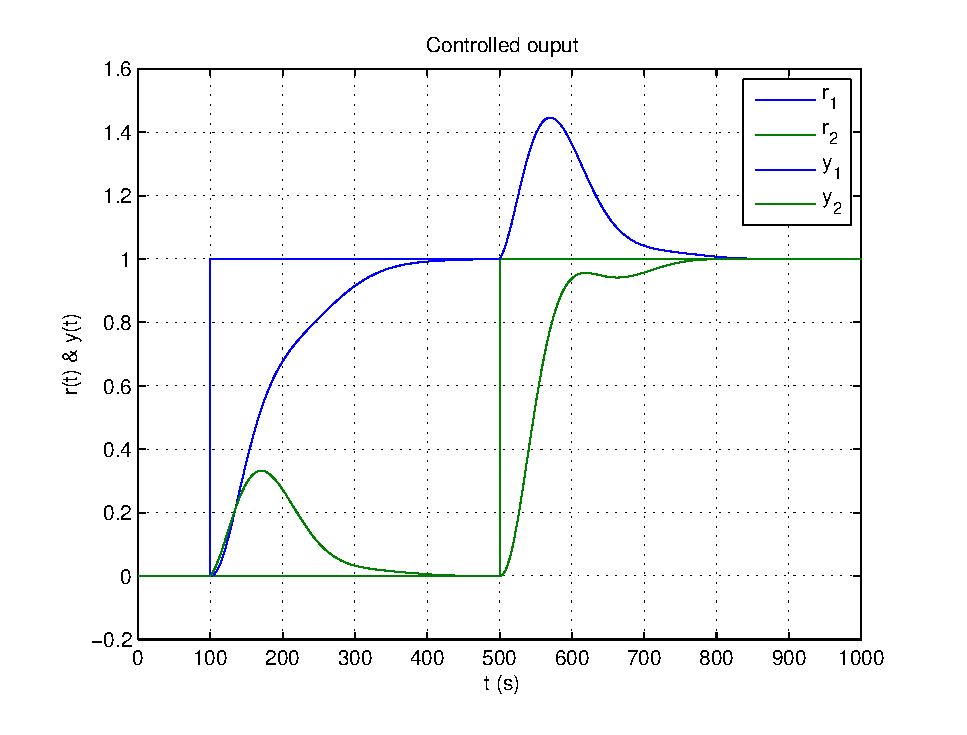
\includegraphics[width=\columnwidth]{fig/controlledouputnm.eps}
    \caption{Response of the non-minimum phase system to $r(t)$}
    \label{simunm}
\end{figure}

\paragraph{Results}

Figure \ref{simum} \& \ref{simunm} shows that the outputs are indeed coupled. 
However the control performance are more satisfying in the minimum-phase case. This is legit since the minimum-phase system do not present a RHP zero.

% \subsubsection{Exercise}

As we have seen in the previous exercise, the control performance are better in the minimum phase case. 
(Even if its a bad idea in most cases to implement a decentralized controller).
Moreover since the non-minimum phase system presents a zero in the RHP it is more complicated to design this kind of controller 



\vspace{.5cm}
\hrulefill
\vspace{.5cm}

\begin{bfseries}
\emph{Conclusion} --
\end{bfseries}

\end{document}
